\documentclass[a4paper,11pt,oneside]{book}
\synctex=1

\usepackage{packages}
\usepackage{frontespizio}
%\makeindex                                          %CREA INDICE ANALITICO

%Document begin
\begin{document}
	%\pagenumbering{roman} %IMPOSTA NUMERAZIONE ROMANA FINO ALL'INTRODUZIONE
	%\afterpage{\cfoot{\thepage}} %METTE I NUMERI DI PAGINA IN FONDO AL FOOTER. NECESSARIO SE SI USA FANCYHDR
	\frontespizio
	%\clearpage{\pagestyle{empty}\cleardoublepage}
	%\setlength{\parskip}{0em}
	\tableofcontents
	%\setlength{\parskip}{1em}
	%\newpage
	%\listoffigures
	\newpage
	%\pagenumbering{arabic} %IMPOSTA NUMERAZIONE TRADIZIONALE A PARTIRE DALL'INTRODUZIONE
	%\pagebreak
	%===========================

	% Numeri vicino alla riga
	% @TODO Rimuovere dopo le correzioni
	\linenumbers

	% \onehalfspacing

	% Introduzione
	% !TEX root=../index.tex

\chapter{Introduzione}
\label{chap:introduction}
    \section{Human Sensing}
    \label{sec:human_sensing}
        L'insieme di tecniche e di soluzioni per il riconoscimento della presenza della persona nello spazio prende il nome \emph{human sensing}.

        Vengono utilizzati vari dispositivi di sensoristica per l'acquisizione di informazioni ai fini del riconoscimento. 
        Dall'elaborazione delle informazioni acquisite, i sistemi di human sensing sono in grado di rilevare la presenza e la posizione della persona all'interno dell'ambiente interessato.

        I contesti applicativi di sistemi di questo genere sono variegati ed in costante espazione.
        Sistemi per il rilevamento delle persone si adattano perfettamente in contesti di sorveglianza, sia al fine di garantire la sicurezza di un ambiente in termini di rilevamento delle intrusioni, sia al fine di costruire delle soluzioni di monitoraggio in ambienti assistivi automatizzati.
        Dispositivi in grado di localizzare corpi umani sono utilissimi nelle attività \emph{search \& rescue}, dove è necessario, in caso di catastrofi o calamità naturali, localizzare nel minor tempo possibile i superstiti in condizioni avverse.
        Vi sono delle applicazioni anche in ambito economico: soluzioni di \emph{people counting} sono sempre più usate nei processi di \emph{business intelligence} per effettuare analisi di mercato.

        Molto spesso, la natura dei sensori utilizzati per le acquisizioni, fanno in modo che i problemi di human sensing si intersechino con problemi di \emph{computer vision}: l'utilizzo di sensori ad acquisizione visiva comporta l'insorgere di svariati problemi di visione artificiale.

        Lo scopo della visione artificiale è quello di riprodurre la vista umana, intesa non come semplice acquisizione di rappresentazione bidimensionale di una regione di spazio, ma mira ad una reale interpretazione del relativo contenuto.

        \subsection{Stato dell'Arte}
            Il crescente interesse per le soluzioni di human sensing ha dato luogo a numerosi studi e ricerche sull'argomento.
            Rimanendo nel contesto del rilevamento legato a problemi di computer vision, spiccano i seguenti risultati.

            \begin{description}
                \item[People Tracking and Counting] \citet{Papageorgiou98} nel \citeyear{Papageorgiou98} proposero una tecnica di riconoscimento e conteggio di pedoni a partire da immagini RGB.
                Elaborando opportunamente le informazioni raccolte da comuni telecamere, il sistema era in grado di apprendere a riconoscere il pattern della figura umana analizzando le variazioni di intensità tra le diverse aree delle immagini.
                Per l'apprendimento utilizzarono una \emph{macchina a vettori di supporto}\footnote{Consultare la sezione \ref{sec:supervised_ensamble_learning} ed in generale tutto il capitolo \ref{chap:adaboost} per ulteriori informazioni al riguardo.}.
                
                \item[Face Recognition] Viola e Jones in \cite{Viola04} descrivono quello che è, ad oggi, il framework più robusto di \emph{object recognition}, applicandolo con successo al caso del riconoscimento dei volti.
                Ancora una volta, si tratta di un sistema allenabile che utilizza l'algoritmo \emph{Adaboost}\footnote{Per maggiori informazioni consultare \cite{Freund97} ed il capitolo \ref{chap:adaboost}.}.

                \item[Human Sensing tramite Kinect] Anche il dispositivo Kinect, prodotto da Microsoft, costituisce, nel complesso, un valido esempio di sistema di human sensing.
                La quantità e la qualità dei sensori con cui è equipaggiato, il costo relativamente basso e la disponibilità di \emph{SDK} e toolkit integrabili con ambienti di sviluppo evoluti, stanno accrescendo la popolarità di tale dispositivo al di là delle applicazioni videoludiche.
                Cresce anche l'interesse per i \emph{serious game}, videogiochi sviluppati con una doppia valenza, quella di assistere e guidare i pazienti in contesti riabilitativi.
            \end{description}

    \section{Panoramica Generale}
    \label{sec:overview}
        Questo elaborato descrive principalmente il lavoro svolto per l'implementazione del sistema di rilevamento descritto da Zhu e Wong in \cite{Zhu13}.
        È correlato di numerosi approfondimenti teorici, necessari, sia per avere una corretta visione d'insieme del problema, sia per essere in grado di agire efficacemente nella futura richiesta di miglioramenti nell'implementazione proposta.

        \subsection{Il Lavoro di Zhu e Wong} % (fold)
        \label{sub:il_lavoro_di_zhu_e_wong}
            Nel \citeyear{Zhu13} Zhu e Wong presentano un sistema di riconoscimento della figura umana, ripresa dall'alto di una stanza, con il dispositivo Kinect.
            Si tratta di una soluzione di human sensing, intercalata in una particolare condizione ambientale, che utilizza il \emph{sensore di profondità} del dispositivo Kinect come sorgente per l'acquisizione di dati.

            Come altre soluzioni proposte in precedenza, il sistema deve essere allenato a riconoscere persone.
            L'algoritmo utilizzato per lo sviluppo dei criteri di riconoscimento è \emph{Adaboost}, lo stesso utilizzato per il framework di \emph{face detection} sviluppato da Viola e Jones.
            Come si potrà vedere in seguito, in maniera più dettagliata, saranno numerose le somiglianze con quest'ultimo.

        \subsection{Configurazione Hardware}
        \label{sub:hardware_configuration}
            Precisamente la versione del dispositivo Kinect utilizzato è la \emph{V2}.
            Il sensore di profondità del Kinect V2 fornisce una rappresentazione bidimensionale dello spazio, fondamentalmente sotto forma di immagini particolari. 
            In queste ultime ogni pixel corrisponde il valore in millimetri della distanza dal sensore della superficie dell'oggetto presente nell'immagine.
            Ci si riferirà ad esse chiamandole \emph{immagini di profondità}.

            Il sensore del Kinect, di cui è disponibile una piccola descrizione più dettagliata all'appendice \ref{chap:kinect}, fornisce uno stream di tali immagini ad una frequenza di 30 frame al secondo: è possibile quindi registrare dei \emph{video di profondità}.

            \subsubsection{Visuale Top-Down}
                Il dispositivo Kinect viene montato al soffitto di una stanza e l'ambiente viene ripreso da tale prospettiva.
                Solitamente l'altezza a cui viene montato è di poco inferiore alla distanza del soffitto dal pavimento (poco meno di $3m$), inoltre la linea focale del sensore dovrebbe essere quanto più possibile ortogonale al pavimento della stanza, in modo da ridurre ai minimi termini la presenza di asimmetrie nelle riprese.
                
                Tali distanze sono perfettamente compatibili con le specifiche tecniche del dispositivo stesso.
                Nel caso in cui vi sia la necessità di montare il Kinect a soffitti più alti di $4m$, si possono utilizzare delle lenti correttive per aumentare il range di affidabilità del sensore.

                Molto sistemi di riconoscimento utilizzano il Kinect - e più in generale, qualsiasi dispositivo di acquisizione visivo - in posizione frontale rispetto ai soggetti da riconoscere.
                Di fatti, il dispositivo, concepito per applicazioni videoludiche, è progettato per operare in tale posizione.
                Tuttavia, la configurazione descritta precedentemente, ha l'enorme vantaggio di eliminare l'occlusione del soggetto: in tali condizioni una persona non può nasconderne dietro di sè un'altra alla vista del sensore (se non in scomode posizioni), cosa invece frequentissima nei i sistemi di rilevamento frontali.

        \subsection{\emph{Head and Shoulders Profile}}
        \label{sub:hasp}
            Riconoscere un oggetto significa mettere in relazione la sua rappresentazione con un concetto, più o meno specifico, che lo descriva.
            In questo caso, dovendo riconoscere delle persone, si dovrà mettere correttamente in relazione un'immagine di profondità che raffigura un individuo con il \emph{concetto di persona}, mentre per un'immagine che non la raffigura, si dovrà evitare una relazione di tale natura.
            
            Si definiscono due classi.
            Il concetto di classe è molto simile a quello delle \emph{classi di equivalenza}, relativo all'algebra astratta, ma anche a quello delle classi come prototipi di \emph{oggetti software}, relativo al paradigma di programmazione ad oggetti.
            Una classe costituisce un insieme di oggetti che condividono determinate proprietà caratteristiche: 
            per le classi di equivalenza, tutti gli elementi appartenenti ad essa devono essere tra di loro in una relazione di equivalenza;
            per le classi software, tutte istanze di tali classi sono caratterizzate dalla medesima struttura (stessi attributi, stessi metodi), anche se poi ogni oggetto è ben distinto dall'altro. 

            Distinguere gli oggetti che rappresentano persone da quelli che non le rappresentano, significa classificare tali oggetti in due classi: la \emph{classe delle persone} e quella delle \emph{non persone}.
            A questo punto, bisogna iniziare a chiedersi quali debbano essere le proprietà degli elementi dell'una e quali quelli dell'altra.

            Bisogna sottolineare il fatto che gli oggetti di una stessa classe, hanno sì delle proprietà in comune tra di loro, ma averne altre per cui differiscono.
            Individuare le \emph{caratteristiche} - ovvero proprietà osservabili e misurabili di un oggetto - in base alle quali decretare l'appartenenza all'una o all'altra classe, non è un problema banale.
            Si può intuire quanto sia vasto l'insieme delle caratteristiche valutabili nella rappresentazione di un oggetto.
            Ovviamente la natura della rappresentazione influisce nella scelta delle caratteristiche più rilevanti.
            
            Si ricordi che un'immagine di profondità rappresenta la realtà attraverso il valore della distanza misurata in ogni punto dello spazio osservato. 
            È naturale, quindi, considerare tali distanze come caratteristiche misurabili dell'oggetto rappresentato.

            In un sistema allenabile, sarà premura del modulo di apprendimento selezionare le caratteristiche più rilevanti per un oggetto.
            Senza anticipare altro sulla questione dell'apprendimento, è comunque utile fornire una descrizione in linguaggio naturale delle caratteristiche della forma del profilo umano, da tale visuale, che saltano immediatamente all'occhio.

            \begin{enumerate}
                \item L'immagine di una persona è caratterizzata da uno \emph{spazio vuoto}\footnote{Per \emph{spazio vuoto} si intende una regione di spazio il cui valore della distanza, percepita dal sensore, è molto vicino al quello della distanza del pavimento della stanza.} di fronte ad essa e dietro di essa.

                \item A sinistra della spalla sinistra ed a destra della spalla destra del profilo dall'alto di una persona, sono presenti degli spazi vuoti.
                
                \item Tra la testa e le spalle vi è una differenza di altezza.
            \end{enumerate}

            Si segua quindi la seguente convenzione: le immagini che soddisferanno le precedenti proprietà saranno chiamate immagini \emph{Head and Shoulders Profile}, o più brevemente \emph{immagini HASP}.

        \subsection{Flusso di Lavoro}
        \label{sub:overall_workflow}
            A conclusione di questa rilassata premessa, per evitare di perdersi in questo miscuglio di osservazioni eterogenee apparentemente prive di uno scopo preciso, è opportuno definire qual è il \emph{workflow} principale dell'intero sistema di rilevamento.
            Sostanzialmente quest'ultimo è diviso in due componenti accoppiati, uno delegato all'apprendimento delle caratteristiche di classificazione, l'altro delegato all'effettivo rilevamento.
            Come è facilmente intuibile, il secondo non può funzionare senza il risultato fornito dal primo, che è il più complesso e corposo dei due.

            \subsubsection{Allenamento}
                Per allenare il sistema è necessario creare un insieme di allenamento, ovvero un insieme i cui elementi sono delle immagini di profondità che ritraggono persone (immagini HASP) e non.
                In fase di creazione, ogni elemento di tale insieme viene dotato di un'etichetta che identifica la reale classe di appartenenza dell'oggetto.

                La componente software che si occupa dell'allenamento del sistema implementa l'algoritmo Adaboost.
                Quest'ultimo riceve in input l'insieme di allenamento, i cui elementi, dotati della rispettiva classificazione reale, sono alla base della scelta delle caratteristiche migliori per la descrizione delle classi di oggetti.
                Alla fine della sua esecuzione, Adaboost restituisce come output un classificatore.

                Nei capitoli successvi si darà una definizione più formale di quello che è un classificatore, per il momento è sufficiente una definizione intuitiva: un classificatore \emph{classifica} i vari oggetti, ovvero fornisce una \emph{previsione} della classe di appartenenza relativamente ad ognuno di essi.

                La classificazione effettuata da questa componente approssima solamente la classificazione reale. 
                La bontà di tale approssimazione sarà il parametro di valutazione della bontà generale del sistema.

                Nel caso di Adaboost il classificatore risultante sarà simile ad una collezione di test: il risultato di tali test, eseguiti su di un qualsiasi oggetto, fornirà la previsione della classificazione dell'oggetto stesso.

            \subsubsection{Rilevamento}
                In questa fase il sistema analizza i frame di profondità delle acquisizione in ordine sequenziale, alla ricerca di persone al suo interno.

                Il classificatore ottenuto al termine dell'esecuzione di Adaboost, sarà in grado di classificare porzioni di immagini di profondità, ma non è in grado di predire direttamente, a partire da un intero frame, la presenza e la posizione di una o più persone al suo interno: le porzioni analizzabili dal classificatore hanno dei vincoli dimensionali da rispettare, che in prima approssimazione si possono immaginare come dei quadrati di dimensione costante.
                L'attività di rilevamento della persona all'interno del frame, quindi, consterà della sequenziale analisi di tutte le porzioni di frame che rispettano tali vincoli, al fine di coprire l'intera area.

                Si vedrà in seguito che nei pressi di una persona nell'immagine di profondità, saranno molteplici le porzioni di frame per le quali il rilevamento darà esito positivo.
                Si pone quindi l'ulteriore problema di selezionare, delle tante porzioni che hanno dato esito positivo, quella che meglio approssima la reale posizione della persona. 


	% Feature di Haar
	% !TEX root=../index.tex

\chapter{Haar-Like Features}
\label{chap:features}
    \section{Definizione}
    \label{sec:haar_features_definition}
        \subsection{Richiamo: cosa è una feature (caratteristica)}
            % @FIXME Possibile ripetizione con sottosezione HASP al capitolo precedente
            % \subsubsection{Cosa sono le caratteristiche di un oggetto}
                Le caratteristiche di un oggetto sono quelle proprietà elementari osservabili e misurabili.

            % \subsubsection{Le caratteristiche dipendono da cosa si vuole evidenziare}
                È stato già detto che la scelta delle caratteristiche è fondamentale e dipende da cosa si vuole mettere in evidenza dell'oggetto in questione.

            % \subsubsection{Le caratteristiche dipendono da cosa si ha a disposizione}
                Ovviamente la scelta delle caratteristiche è sempre subordinata a ciò che si ha disposizione.
        \subsection{Wavelet di Haar}
            \subsubsection{Le feature di Haar derivano dalle wavelet di Haar}
                Le feature di Haar si adattano molto bene alle proprietà che si vogliono misurare degli oggetti appartenenti all'applicazione d'interesse.
                Sono un costrutto derivante dalle \emph{wavelet di Haar}.
            \subsubsection{Definizione informale delle wavelet di Haar}
                % \paragraph{Chi le ha sviluppate}
                Alfréd Haar sviluppò il primo tipo di wavelet.

                % \paragraph{Cosa sono (base ortonormale spazio funzionale)}
                Furono sviluppate come un esempio di funzioni ortonormali di base per uno spazio funzionale.

                % \paragraph{Rappresentazione dei segnali (fourier duale)}
                In quanto base di uno spazio ortornomale, con le wavelet di Haar è possibile esprimere un qualsiasi segnale limitato.
                Esse costituiscono, sotto particolari ipotesi, un sistema di rappresentazione dei segnali duale all'analisi spettrale di Fourier.
                Hanno anche il vantaggio, rispetto a quest'ultimo, di mantenere l'informazione del tempo (approfondire).

            \subsubsection{Wavelet di Haar e DWT}
                % \paragraph{DWT}
                Le wavelet di Haar sono state utilizzate nelle \emph{Discrete Wavelet Transform}, in breve DWT.

                % \paragraph{Utilizzi commerciali DWT (JPEG2000)}
                Un'importante applicazione delle DWT è quella definita dal nuovo standard di compressione delle immagini JPEG2000.

                % \paragraph{Utilizzo delle dwt per il pattern recognition}
                Nelle applicazioni di machine learning e pattern recognition, le trasformazioni DWT furono utilizzate nei primi lavori di riconoscimento a partire da immagini RGB (riconoscimento dei pedoni).
                È da quest'ultima applicazione che hanno origine le feature di Haar come verranno trattate.

        \subsection{Formula di calcolo standard}
            \subsubsection{Rappresentazione visuale}
            Le feature di Haar sono rappresentabili come due aree adiacenti, una chiara ed una scura.
            La somma delle intensità (il valore numerico) di tutti i pixel dell'area scura, viene sottratta alla somma delle intensità di tutti i pixel nell'area chiara.
            Ciò permette di evidenziare le differenze di intensità medie tra i valori dei pixel nelle due aree.
            [Formula a due aree]
            È da notare il fatto che, con le feature di Haar, non si vanno a valutare i singoli pixel al fine di individuarne un pattern, ma si ragiona procedendo per aree adiacenti.

            \subsubsection{Formula generale}
            La definizione delle feature di Haar può essere estesa all'utilizzo di più di due aree adiacenti.
            Il principio resta lo stesso: si hanno due gruppi di aree, uno chiaro ed uno scuro.
            La formula di calcolo si generalizza con estrema semplicità.
            [Formula generale con più aree]

            \subsubsection{Altri tipi di feature (OpenCv)}
            È possibile formulare feature di moltissime formule.
            La libreria di computer vision OpenCV mette a disposizione una grande varietà di feature, introducendo anche quelle la cui forma è inclinata di 45°. (Citare articolo in cui vi è la definizione delle feature a 45°).

            \subsubsection{Tipi di feature utilizzate}
            In questa applicazione vengono utilizzati solo due 4 tipi di feature, contro i 5 utilizzati nel sistema di riconoscimento di Viola-Jones.

        \subsection{Cosa mette in evidenza la feature di Haar}
            \subsubsection{Immagini normali (Viola Jones)}
            Nella framework di riconoscimento dei volti di Viola-Jones, le immagini RGB sono la fonte di informazioni del sistema.
            Vengono applicate le feature di Haar a tali immagini (ovviamente dopo che queste ultime sono state trattate da opportune operazioni di preprocessing) e ciò che viene evidenziato sono le differenze di intensità tra le regioni della foto.
            A far variare l'intensità di un pixel in una foto concorrono l'illuminazione, il colore e molti altri fattori.
            Tuttavia, le feature di Haar divengono il mezzo con il quale si può riconoscere un volto umano.
            Ad esempio, è stato osservato che nella foto di un volto, l'area che racchiude entrambi gli occhi e l'inizio del naso è caratterizzato da una particolare variazione di luminosità, misurabile e utilizzabile per descriminare le i volti da i non volti.

            \subsubsection{Immagini di profondità (Zhu Wong)}
            Nelle immagini di profondità, dove il valore di ogni pixel corrisponde alla distanza in millimetri della superficie dal sensore, applicare le feature di Haar ad un'area dell'immagine equivale a misurare le differenze di quota tra due aree adiacenti tra di loro.
            Il sistema di allenamento deciderà quali sono le feature migliori per il riconoscimento della persona, ma tutto si basa sul concetto che le differenze di quota osservabili dal profilo ripreso dall'alto di una persona sono caratteristiche della persona stessa e costituiscono il parametro di riconoscimento rispetto ad un qualsiasi altro oggetto.
            Una sedia, un tavolo o qualsiasi altro elemento presenterà delle differenze di quota differenti dal profilo della persona.

        \subsection{Formula di calcolo invariante ai resize}
            \subsubsection{Anticipazione del problema del ridimensionamento}
            In seguito sarà necessario ridimensionare una feature in modo da coprire un'area più grande, in quanto, dovendo misurare le caratteristiche degli oggetti di interesse, questi ultimi sono variabili in dimensione.
            Il valore calcolato con la feature in questione, tuttavia, non dovrebbe essere troppo sensibile ai ridimensionamenti (che saranno frequenti).

            \subsubsection{Formula: Normalizzazione sull'area}
            Al fine di ottenere la massima invarianza ai ridimensionamenti dell'area della feature, il valore di essa viene normalizzato con l'estensione dell'area totale valutata.
            [Formula normalizzata]

        \subsection{Vantaggi}
            \subsubsection{Differenze di intensità vs Valutazione dei singoli pixel}
            Il primo indiscutibile vantaggio delle feature di Haar sta nel fatto che la caratterizzazione dell'oggetto viene effettuata sulla base di osservazioni d'insieme su intere aree dell'immagine e non su ossevazioni globali effettuate su singoli pixel.
            Oltre alla grandissima complessità che una valutazione su singoli pixel introdurrebbe, bisogna prendere atto che, con dati soggetti a disturbi e alla presenza di rumore, delle caratteristiche misurate sui singoli pixel non sarebbero molto significative.

            \subsubsection{Differenze di intensità vs Estrazione dei contorni}
            L'estrazione dei contorni potrebbe essere più significativo della valutazione sui singoli pixel, ma continuano ad essere caratteristiche abbastanza complesse da calcolare ed ottenere.
            L'estrazione dei contorni, inoltre, è un concetto fortemente legato alle immagini RGB, usarlo con le immagini di profondità è un forzatura.

            \subsubsection{Estrema efficienza computazionale}
            Il principale vantaggio delle feature di Haar rispetto ad altri tipi più elaborati di feature resta la loro efficienza computazionale.
            Si vedrà che, con una particolare struttura dati di supporto, calcolare il valore di un feature di Haar per un'immagine è un'operazione eseguibile in un tempo costante.
    \section{Immagine Integrale}
    \label{sec:integral_image}
        \subsection{Definizione rigorosa dell'immagine integrale}
            \subsubsection{Problema: efficienza nel calcolo di somme di pixel}
                % \paragraph{Complessità computazionale del calcolo \emph{ignorante}}
                Il calcolo della somma delle intensità di ciascun pixel appartenente ad un'area, necessario al fine di calcolare il valore delle feature di Haar, è un'operazione il cui costo varia all'aumentare della dimensione complessiva dell'area.
                Calcolare tali somme infatti ha complessità computazionale $\Theta(m \cdot n)$ con $m$ ed $n$ dimensione dell'area.

                % \paragraph{Soluzione: rendere queste somme subito disponibili}
                La soluzione a tale problema consiste nell'utilizzo dell'immagine integrale, una struttura dati che mette a permette di calcolare la somma dei pixel di qualsiasi area all'interno di essa in un tempo costante.
            \subsubsection{Definizione immagine integrale}
                Un'immagine integrale è un matrice delle stesse dimensioni dell'immagine di partenza.
                Ogni elemento di tale matrice contiene il valore della somma dei pixel che si trovano al di sopra e a destra (estremi inclusi) del pixel relativo alla posizione dell'elemento.
                [Formula]
            \subsubsection{Formula di calcolo della somma dei pixel in un'area}
                % \paragraph{Enunciazione della formula}
                Attraverso l'immagine integrale è possibile calcolare l'area necessaria per una feature sommando i valori dei due vertici dell'area sulla diagonale principale e sottrandovi quelli dei vertici sulla diagonale secondaria.
                [Formula]

                % \paragraph{Dimostrazione della formula}
                [Dimostrazione formula]

                % \paragraph{Complessità computazionale del calcolo della feature}
                Qualsiasi calcolo di questo tipo richiederà un tempo costante, non più legato alle dimensioni dell'input.
                La complessità computazionale è quindi $\Theta(1)$.

        \subsection{Complessità computazionale generale}
            \subsubsection{Complessità del calcolo dell'immagine integrale}
            La complessità computazione totale del calcolo dell'immagine integrale continua ad essere legata alla dimensione dell'input.
            Se l'immagine è larga $w$ pixel ed alta $h$ pixel, la complessità computazionale per la generazione dell'immagine integrale è pari a $\Theta(w \cdot h)$.

            \subsubsection{Convenienza del calcolo dell'immagine integrale}
            L'utilizzo delle immagini integrale è molto vantaggiosa nel momento in cui è necessario calcolare molte feature sulla stessa immagine.
            Volendo essere più espliciti, se la complessità computazionale totale del calcolo di $n$ feature senza l'utilizzo dell'immagine integrale è maggiore di quella per la generazione dell'immagine integrale stessa, allora è vantaggioso utilizzare tale struttura dati.

    \section{Decision Stump}
    \label{sec:decision_stump}
        \subsection{Problema: utilizzare le feature}
            % \subsubsection{È necessario un meccanismo primitivo per utilizzare le feature}
            Una volta misurata una caratteristica di un oggetto, bisogna essere in grado di utilizzarla ai fini di classificarlo.

            % \subsubsection{Bisogna discriminare in base al valore}
            È necessario, quindi, un meccanismo per effettuare una previsione della classe di appartenenza dell'oggetto che si basa esclusivamente sul valore della feature misurata.

        \subsection{Definizione di albero decisionale}
        Un albero decisionale è un modello predittivo. Ogni nodo dell'albero rappresenta una variabile o una proprietà osservabile. Ogni arco dal nodo padre verso un nodo figlio rappresenta un possibile valore per la proprietà del nodo padre. Le foglie dell'albero rappresentano i valori che si predice possa assumere una variabile obiettivo. Il percorso dalla radice ad una foglia rappresenta la previsione del valore di tale variabile obiettivo a fronte delle osservazioni effettuate sui valori delle variabili rappresentate da ciascun nodo attraversato.
        \subsection{Definizione di decision stump} % @TODO Finire questa sottosezione
            \subsubsection{Radice: Test, funzione booleana}
            Il più semplice albero decisionale è il \emph{decision stump}. Ha profondità unitaria, cioè si basa sull'osservazione di una sola variabile, in base al valore della quale può effettuare due diverse previsioni della variabile obiettivo (ha due foglie).
            \subsubsection{Foglie: risultati possibili}
            \subsubsection{Formule di calcolo binaria}
            \subsubsection{Formula di calcolo unica: polarità}


	% !TEX root=../index.tex

% Capitoli sviluppati fino al 5° livello di profondità
% Introduzione

\chapter{Haar-Like Features}
\label{chap:features}
    \section{Definizione}
    \label{sec:haar_features_definition}
        \subsection{Richiamo: cosa è una feature (caratteristica)}
            \subsubsection{Cosa sono le caratteristiche di un oggetto}
            \subsubsection{Le caratteristiche dipendono da cosa si vuole evidenziare}
            \subsubsection{Le caratteristiche dipendono da cosa si ha a disposizione}
        \subsection{Wavelet di Haar}
            \subsubsection{Le feature di Haar derivano dalle wavelet di Haar}
            \subsubsection{Definizione informale delle wavelet di Haar}
                \paragraph{Chi le ha sviluppate}
                \paragraph{Cosa sono (base ortonormale spazio funzionale)}
                \paragraph{Rappresentazione dei segnali (fourier duale)}
            \subsubsection{Wavelet di Haar e DWT}
                \paragraph{Utilizzi commerciali DWT (JPEG2000)}
                \paragraph{Utilizzo delle dwt per il pattern recognition}
        \subsection{Formula di calcolo standard}
            \subsubsection{Rappresentazione visuale}
            \subsubsection{Formula generale}
            \subsubsection{Altri tipi di feature (OpenCv)}
            \subsubsection{Tipi di feature utilizzate}
        \subsection{Cosa mette in evidenza la feature di Haar}
            \subsubsection{Immagini normali (Viola Jones)}
            \subsubsection{Immagini di profondità (Zhu Wong)}
        \subsection{Formula di calcolo invariante ai resize}
            \subsubsection{Anticipazione del problema del ridimensionamento}
            \subsubsection{Formula: Normalizzazione sull'area}
        \subsection{Vantaggi}
            \subsubsection{Differenze di intensità vs Valutazione dei singoli pixel}
            \subsubsection{Differenze di intensità vs Estrazione dei contorni}
            \subsubsection{Estrema efficienza computazionale}
    \section{Immagine Integrale}
    \label{sec:integral_image}
        \subsection{Definizione rigorosa dell'immagine integrale}
            \subsubsection{Problema: efficienza nel calcolo di somme di pixel}
                \paragraph{Complessità computazionale del calcolo \emph{ignorante}}
                \paragraph{Soluzione: rendere queste somme subito disponibili}
            \subsubsection{Definizione immagine integrale}
            \subsubsection{Formula di calcolo della somma dei pixel in un'area}
                \paragraph{Enunciazione della formula}
                \paragraph{Dimostrazione della formula}
                \paragraph{Complessità computazionale del calcolo della feature}
        \subsection{Complessità computazionale generale}
            \subsubsection{Complessità del calcolo dell'immagine integrale}
            \subsubsection{Convenienza del calcolo dell'immagine integrale}
    \section{Decision Stump}
    \label{sec:decision_stump}
        \subsection{Problema: utilizzare le feature}
            \subsubsection{È necessario un meccanismo primitivo per utilizzare le feature}
            \subsubsection{Bisogna discriminare in base al valore}
        \subsection{Definizione di albero decisionale}
        \subsection{Definizione di decision stump}
            \subsubsection{Radice: Test, funzione booleana}
            \subsubsection{Foglie: risultati possibili}
            \subsubsection{Formule di calcolo binaria}
            \subsubsection{Formula di calcolo unica: polarità}

\chapter{L'Algoritmo di Allenamento: Adaboost}
\label{chap:adaboost}
    \section{Apprendimento Supervisionato \emph{Ensamble}}
    \label{sec:supervised_ensamble_learning}
        \subsection{Apprendimento Supervisionato}
        \label{sub:supervised_learning}
            \subsubsection{Definizione}
                \paragraph{Obiettivo}
                \paragraph{Spazio delle Ipotesi}
            \subsubsection{Esempi di Supervised learning}
                \paragraph{Algoritmi di Sup.Learning}
                \paragraph{Maggiori campi applicativi}
                \paragraph{Concetti di base}
                    \subparagraph{Overfitting}
            \subsubsection{Ensamble Learning}
        \subsection{\emph{Adaptive Boosting}}
        \label{sub:adaptive_boosting}
            \subsubsection{Algoritmi di Boosting}
            \subsubsection{Aptive: adattabilità}
            \subsubsection{Strong learner e Weak learner}
    \section{Dataset di Allenamento}
    \label{sec:training_dataset}
        \subsection{Categorie di Classificatori}
        \label{sub:classifiers_categories}
            \subsubsection{Variabilità della forma HASP}
                \paragraph{Variazione dell'orientazione}
                \paragraph{Variazione derivata dalla distorsione prospettica}
            \subsubsection{Definizione delle categorie di classificatori}
                \paragraph{Categorie: Verticale e Orizzontale}
                \paragraph{Categorie alternative: Obliquo, a zone}
        \subsection{Preparazione dei Dataset}
        \label{sub:datasets_setup}
            \subsubsection{Acquisizioni}
                \paragraph{Soggetti, percorsi}
                \paragraph{Acquisizione delle registrazioni}
            \subsubsection{Ritaglio dei samples}
                \paragraph{Trainset Creator}
        \subsection{Preprocessing}
        \label{sub:preprocessing}
            \subsubsection{Resize}
                \paragraph{Nearest Neighbour}
                \paragraph{Altri algoritmi di resize}
            \subsubsection{Conversione delle distanze}
    \section{\emph{Strong Learner}}
    \label{sec:strong_learner}
        \subsection{Procedura di estrazione del classificatore forte}
    \section{\emph{Weak Learner}}
    \label{sec:weak_learner}
        \subsection{Procedura di estrazione del classificatore debole}
        \subsection{Valutazione della complessità computazionale}

% Valutare l'accorpamento dei due capitoli successivi
\chapter{Validazione e Regolazione dei Classificatori}
\label{chap:tuning}
    \section{Criteri di Valutazione}
    \label{sec:evaluation_criteria}
    \section{Dataset di Validazione}
    \label{sec:validation_dataset}
        \subsection{Criteri di creazione delle registrazioni}
        \subsection{Altre caratteristiche}
    \section{Massimizzazione all'\emph{Accuracy}}
    \label{sec:accuracy_maximization}
        \subsection{Parametri liberi del classificatore}
            \subsubsection{Numero di weak learner}
            \subsubsection{Soglia del classificatore}
        \subsection{Algoritmo di ricerca della soglia e del NWL ottimi}
    \section{Analisi dei Risultati}
    \label{sec:Analisi dei Risultati}

\chapter{Rilevamento}
\label{chap:rilevamento}
    \section{Tecnica di Rilevamento}
    \label{sec:detection_tecnique}
        \subsection{Detection Window}
        \subsection{Rilevazione su frame}
            \subsubsection{Resize detection window}
            \subsubsection{Slide detection window}
    \section{Selezione della Finestra Migliore} %@TODO
    \label{sec:best_detection_window}
        \subsection{Introduzione al problema}
        \subsection{Algoritmo di selezione}
    \section{Confronto con l'Algoritmo G-C} %@TODO
    \label{sec:gc_algorithm_comparison}

\chapter{Conclusioni}

% Questa parte non è stata ancora analizzata
\begin{appendices}
    \chapter{Software Sviluppato}
    \label{chap:software}
        \section{Componenti}
            \subsection{Creatore dei Dataset}
            \subsection{Allenamento}
            \subsection{Tuning, Testing, Rilevamento}
        \section{Tecnologie utilizzate}
            \subsection{C++ e Matlab}
            \subsection{Git e Github [Opzionale]}
        \section{Proposte di miglioramento}

    \chapter{Cenni del funzionamento del sensore Kinect}
    \label{chap:Cenni del funzionamento del sensore Kinect}
\end{appendices}


	% Introduzione
	% % !TEX root=../index.tex

\section{Introduzione}
\label{sec:Introduzione}
    Introduzione di carattere generale: human sensing, visione artificiale, importanza delle soluzioni di rilevamento umano e contesti applicativi.

    Stato dell'arte di ampio spettro: face-detection, pedestrian-detection, ecc

    Obiettivo: riferimenti a \cite{Zhu13}, vantaggi del setup top-down

    \cite{Zhu13}

    Setup: descrizione del setup hardware e software

    Presentazione della tesi: descrizione puntuale dei capitoli successivi


	% Questa sezione va accorpata a quella precedente
	% % !TEX root=../index.tex

\chapter{Panoramica del sistema}
\label{cap:overview}
Riproducendo la configurazione proposta in \cite{Zhu13} al soffitto del laboratorio è stato fissato un dispositivo Kinect V2 rivolto verso il pavimento.
In tale configurazione, all'ingresso di una persona nella visuale del Kinect, ne saranno ben visibili la testa e le spalle.

\section{Il Kinect}
\label{sec:sensor}
Ad onor del vero, ciò che viene comunemente chiamato \emph{sensore di profondità} (o sensore di distanza) del Kinect, è in realtà uno \emph{scanner 3D a luce strutturata}\footnote{Nonostante ciò, lo si continuerà a chiamare \emph{sensore di profondità}, leggermente inesatto, ma decisamente più breve ed intuitivo}.
\begin{wrapfigure}{r}{}
    \begin{center}
        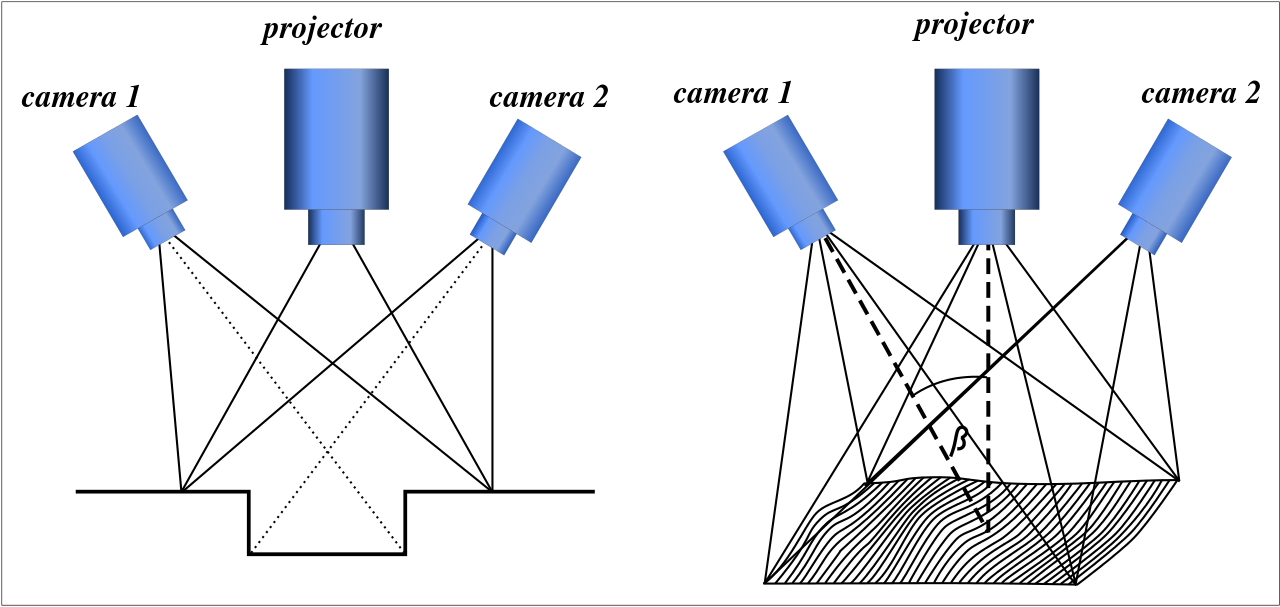
\includegraphics[width=8cm]{img/3d-structured-light-scanner.png}
    \end{center}
    \label{fig:structured_light_scanner}
    \caption{Schematizzazione di uno scanner 3D a luce strutturata.}
\end{wrapfigure}
Un sorgente di raggi infrarossi proietta una serie di pattern codificati. La deformazione indotta dalle superfici degli oggetti interessati viene acquisita da una o più telecamere ed utilizzata per il calcolo delle coordinate tridimensionali.

Il risultato di un sensore di questo tipo è un insieme di triplette $(x,y,z)$, organizzate in una \emph{immagine di profontità}, una struttura dati che è molto simile ad una semplice immagine in scala dei grigi, dove il valore di ogni pixel rappresenta la misura in millimetri della distanza della superficie dal sensore.
La forte somiglianza con le immagini in scala dei grigi è supportata dal fatto che ogni pixel è codificato utilizzando 16bit.

La massima affidabilità del sensore del Kinect si ha per distanza comprese tra $50cm$ e $4,5m$.
Il dispositivo è montato al soffitto a $2,8m$ da terra e ha un campo visivo di $70^{\circ} \times 60^{\circ}$, il quale, all'altezza del pavimento, determina un'area di cattura di circa $4m \times 5m$.

La dimensione di ogni immagine di profondità è di $512 \times 424$ pixel. Nativamente non vengono codificate in alcun modo particolare, sono delle semplici matrici di interi.
Il Kinect V2 è in grado di catturarne fino a 30 al secondo. Utilizzando un apposito software di registrazione è stato possibile mettere insieme dei video di profondità a 30 fps.

\section{Head and Shoulder Profile}
\label{sec:hasp}

\begin{wrapfigure}{l}{}
    \begin{center}
        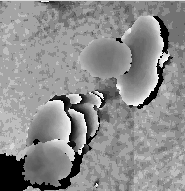
\includegraphics[width=5cm]{img/no_occlusion.png}
    \end{center}
    \caption{Due persone in un ritaglio proveniente da un frame di profondità. Il frame è stato acquisito con il Kinect V1, a differenza di quello in figura \ref{fig:spatial_feature}, acquisito con il Kinect V2.}
    \label{fig:no_occlusion}
\end{wrapfigure}

In condizioni ottimali, la figura umana ripresa dall'alto è composta solamente dalla testa e dalle spalle.
Finchè si trova quasi in corrispondenza del sensore, nella parte centrale dell'immagine di profondità, la restante parte del corpo rimane quasi del tutto nascosta. Sulla posizione delle braccia non si possono fare delle assunzioni precise.

In figura \ref{fig:no_occlusion}, la figura dell'individuo a destra corrisponde a tale descrizione, mentre dell'altro è visibile parte del corpo ed una delle due spalle è nascosta dalla testa.
Nelle zone periferiche di un frame di profondità, l'immagine è soggetta alla \emph{distorsione prospettica} così come lo è quella di qualunque telecamere RGB.

Tale distorsione costituisce un disturbo, dal momento che la figura dello stesso soggetto varia a seconda della relativa posizione nell'area di visualizzazione.
Si vedrà più avanti come affrontare tale situazione, per il momento si considerano solamente le immagini proveniente dalle zone centrali dei frame (come quella in figura \ref{fig:spatial_feature}).

Un grande vantaggio dell'utilizzo del Kinect in questa configurazione è l'\emph{assenza di occlusione}.
Infatti, rispetto ai molteplici sistemi di riconoscimento frontali, i soggetti non possono nascondersi l'uno con l'altro al sensore.

Utilizzare le immagini di profondità significa ragionare con le distanze: piuttosto che cercare di descrivere l'immagine del profilo umano in termini di forma, deve essere descritto in termini di differenze di quota rispetto all'ambiente circostante.
Alla luce di ciò, si possono identificare i seguenti criteri descrittivi:

\begin{enumerate}
    \item L'immagine di una persona è caratterizzata da uno spazio vuoto di fronte ad essa e dietro di essa. Per \emph{spazio vuoto} si intende una regione la cui distanza dal sensore è circa quella del pavimento.
    \item A sinistra della spalla sinistra ed a destra della spalla destra del profilo dall'alto di una persona, sono presenti degli spazi vuoti.
    \item Tra la testa e le spalle vi è una differenza di altezza.

\end{enumerate}

\begin{wrapfigure}{r}{}
    \begin{center}
        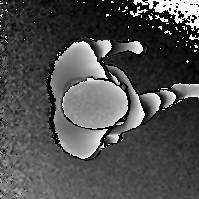
\includegraphics[width=4cm]{img/spatial_features.png}
    \end{center}
    \caption{Una persona mentre cammina}
    \label{fig:spatial_feature}
\end{wrapfigure}

Di qui in avanti, con l'acronimo \emph{HASP} (\emph{Head And Shoulder Profile}), ci si riferirà proprio al profilo della persona ripreso dall'alto che soddisfa i criteri appena elencati.

\section{Un problema di Classificazione} % (fold)
\label{sub:struttura_software}
Il software è diviso in due moduli: il modulo per il riconoscimento e il modulo di allenamento.

Nella prima fase, quella di allenamento, il relativo modulo software, a partire da un insieme di campioni classificati, genererà un insieme di regole per classificare campioni con le medesime caratteristiche. Implementa l'algoritmo Adaboost.

La seconda fase, quella di riconoscimento, lavora su dati reali: ad ogni frame acquisito tramite il sensore di profondità del Kinect si applicano le regole di classificazione generate nella fase precedente, stabilendo se nel frame è stata ripresa una persona e - in caso affermativo - la posizione di quest'ultima.


	% % !TEX root=../index.tex

\chapter{Haar-like Features}
\label{cap:haar_features}
\emph{Definizione delle feature.
Derivazione delle feature dalle wavelet di Haar.
Immagini integrali.
Decision Stump.} 


La descrizione di un qualsiasi oggetto avviene attraverso la descrizione dei suoi attributi. La forma geometrica, le dimensioni, il peso, il colore sono solo una manciata dei possibili attributi con i quali descrivere un oggetto.
L'essere umano è dotato di 5 sensi attraverso i quali è in grado di \emph{percepire} la realtà circostante e di un'infinità di modi con cui \emph{descriverla}.

Il riconoscimento di un oggetto avviene solo in un secondo momento, attraverso l'analisi della sua descrizione, valutando gli attributi che, in quel contesto, sono più signicativi.
Nell'ambito della visione artificiale, il riconoscimento degli oggetti segue esattamente lo stesso flusso.
Gli attributi di un oggetto vengono descritti mediante l'utilizzo di \emph{feature}, ovvero dei meccanismi per misurare le varie proprietà dell'oggetto stesso.

Le immagini di profondità sono il frutto della percezione della realtà, le feature di Haar costituiscono gli attributi con i quali è possibile descrivere tali immagini.


\section{Definizione}
\label{sec:haar_def}
Le feature di Haar riescono a misurare la quantità e il verso delle variazioni di intensità tra due regioni adiacenti di una immagine.
La comune rappresentazione grafica di tali feature mette in evidenza le due regioni colorandone una bianco e l'altra di nero.
La somma delle intensità dei pixel della regione bianca a cui viene sottratta la somma delle intensità della regione nera fornisce una misura della variazione media di intensità tra le due regioni (equazione \ref{eq:haar_feature_informal}).

Di feature ne esistono di diverse forme: in figura \ref{fig:features_type} sono presenti quelle utilizzate in questo ambito, ma disponibili molte forme di feature utilizzate da altri sistemi di object detection. Non tutte sono formate solamente da \emph{due regioni adiacenti}, ma l'importante è che tutte abbiano una regione \emph{nera} ed una regione \emph{bianca}.

\begin{wrapfigure}{L}{0cm}
    \centering
    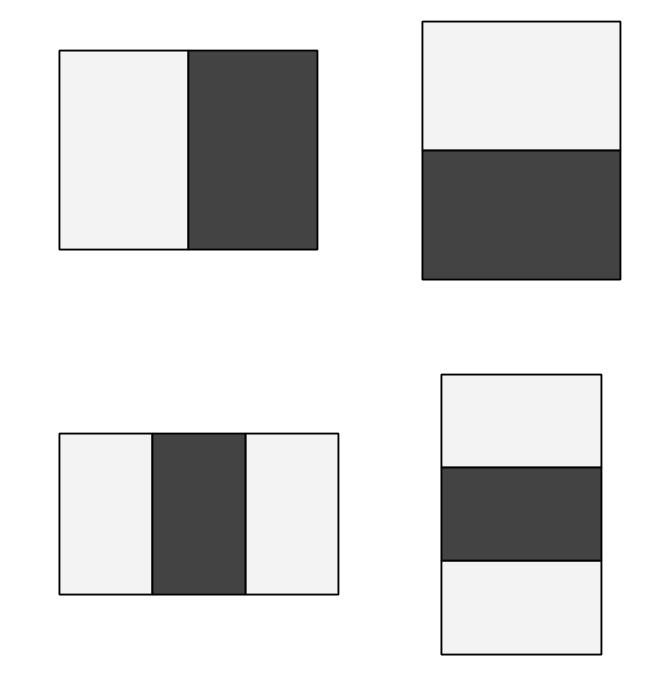
\includegraphics[width=5cm]{img/feature_types.jpg}
    \caption{Tipi di feature di Haar utilizzati in \cite{Zhu13}.}
    \label{fig:features_type}
\end{wrapfigure}

L'equazione \ref{eq:haar_feature_informal} fornisce una descrizione informale del funzionamento delle feature di Haar. Con $E(Area)$ si intende la somma delle intensità di tutti i pixel che appartengono all'area specificata.

\begin{equation}
    f(Img) = E(Area_{white}) - E(Area_{black})
    \label{eq:haar_feature_informal}
\end{equation}

Il segno del valore di una feature identifica il verso della variazione. Se si prende in esame la forma di feature in alto a sinistra della figura \ref{fig:features_type}, un valore positivo denota un'intensità mediamente maggiore nella regione bianca rispetto alla media della regione nera e viceveresa.

Evidenziare le variazioni di intensità delle immagini integrali attraverso l'applicazione delle feature di Haar equivale ad evidenziare le differenze di quota medie delle regioni individuate dalla feature e questo le rende particolarmente adatte a questa applicazione.

In seguito sarà necessario dover calcolare gruppi di feature in diverse scale. Ridimensionare un gruppo di feature è una cosa semplice e verrà trattata in seguito, ma affinchè il valore della feature sia il meno possibile sensibile ai ridimensionamenti è necessario rapportare tale valore all'estensione totale dell'area interessata (equazione \ref{eq:haar_scale_invariant}).

\begin{equation}
    f'(Img) = \frac{E(Area_{white}) - E(Area_{black})}{size(Area_{white}) + size(Area_{black})}
    \label{eq:haar_scale_invariant}
\end{equation}

\section{Dalle Wavelet di Haar alle Feature}
\label{sec:haar_wavelet}
Le feature di Haar derivano dall'estensione bidimensionale delle wavelet di Haar, che sono il primo esempio di wavelet e vennero sviluppate nel 1909 da Alfrèd Haar \cite{Haar10}.
La wavelet madre (equazione \ref{eq:mother_wavelet}) è una funzione oscillante di lunghezza finita, caratteristica comune a tutti i tipi di wavelet.

\begin{equation}
\label{eq:mother_wavelet}
    \psi(x) =
    \begin{cases}
        1 & 0 \leq t < 1/2 \\
        -1 & 1/2 \leq t < 1 \\
        0 & \text{ altrimenti }
    \end{cases}
\end{equation}

Ogni segnale può essere rappresentato per mezzo delle wavelet di Haar. Costituiscono un sistema di rappresentazione duale alla serie di Fourier.

\begin{figure}[!htb]
    \minipage{0.45\textwidth}
    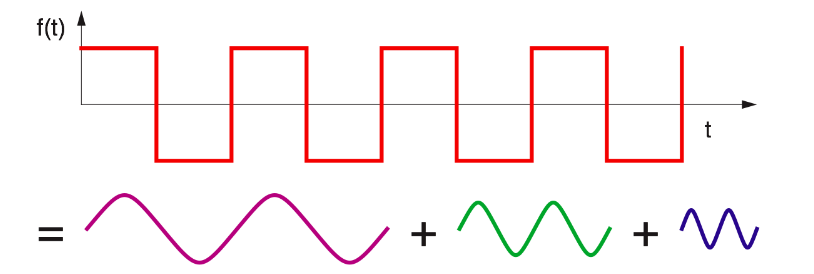
\includegraphics[width=\linewidth]{img/fourier_rapresentation.png}
    \caption{Rappresentazione di un segnale con una serie di funzioni armoniche.}
    \label{fig:awesome_image1}
    \endminipage\hfill
    \minipage{0.45\textwidth}
    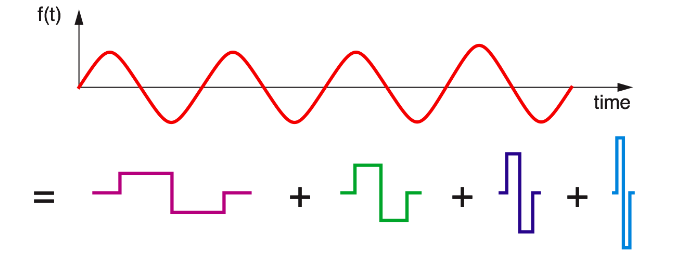
\includegraphics[width=\linewidth]{img/haar_rapresentation.png}
    \caption{Rappresentazione di un segnale con una serie di wavelet di Haar.}
    \label{fig:awesome_image2}
    \endminipage
\end{figure}

Alfrèd Haar propose anche la prima DWT (\emph{Discrete Wavelet Transform}) con la quale, le wavelet che compongono un segnale, vengono campionate discretamente.
Le applicazioni sono notevoli e ad ampio spettro, prime tra tutte quelle nell'ambito della codica dei segnali e nella compressione dei dati. Per fare un esempio, lo standard di compressione JPEG2000 sfrutta la trasformazione DWT \cite{Jpeg2000} per ottenere risultati qualitativamente migliori rispetto allo standard precedente.

Una variante della trasformazione DWT con le wavelet di Haar bidimesionali (figura \ref{sec:haar_wavelet}) è stata utilizzata da \citet{Oren97} in un sistema in grado di riconoscere la presenza di pedoni in delle immagini.

\begin{wrapfigure}{L}{0cm}
    \centering
    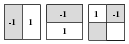
\includegraphics[width=3cm]{img/haar_wavelet.png}
    \caption{Wavelet di Haar bidimensionali utilizzate in \cite{Oren97}.}
    \label{fig:haar_wavelet}
\end{wrapfigure}

Applicando alle immagini la trasformata DWT in diverse scale, si passa da una rappresentazione dell'immagine in scala dei grigi, ad una rappresentazione in termini di coefficienti delle wavelet di Haar.
Tali coefficienti denotano le differenze di intensità tra le aree adiacenti dell'immagine e vengono utilizzati per evidenziare analogie strutturali delle immagini che contengono la figura di un pedone.

\begin{wrapfigure}{R}{0cm}
    \centering
    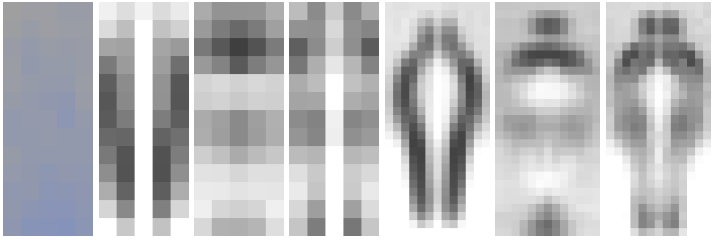
\includegraphics[width=8cm]{img/pedestrian_dwt.png}
    \caption{Coefficienti delle wavelet di trasformate DWT di diverse scale applicate alla stessa immagine. I coefficienti vengono codificati utilizzando la scala dei grigi \cite[Figura 3]{Oren97}.}
    \label{fig:non_standard_dwt}
\end{wrapfigure}

Nella descrizione di un framework generale per l'object detection, \citet{Papageorgiou98} utilizzano la trasformata DWT a wavelet di Haar bidimensionali non per l'estrazione di un template dell'oggetto espresso in variazioni di intensità, bensì per la selezione delle wavelet più significative al fine del riconoscimento dell'oggetto.

Una wavelet di Haar bidimensionale di una data dimensione, utilizzata per campionare un'immagine in una posizione specifica mette in evidenza le differenze di intensità dell'immagine nella regione descritta dall'area della wavelet. Tale differenza di intensità costituisce una proprietà osservabile e misurabile dell'immagine che ritrae l'oggetto. Queste sono le \emph{Haar-like feature} (o semplicemente feature di Haar).

\section{Immagine Integrale}
\label{sec:integral_image}
Le feature di Haar vengono utilizzate anche nel riconoscimento dei volti umani di Viola-Jones.
Sono molto apprezzate, sebbene siano molto primitive rispetto ad altri tipi più evoluti di feature, per la loro efficienza computazionale.

Il calcolo della somma delle intensità dei pixel di un'area è un'operazione il cui costo aumenta linearmente con la quantità di pixel. Introducendo il concetto di \emph{immagine integrale}, ottenuta rielaborando l'immagine di partenza, tale somma viene eseguita una volta per ogni immagine, permettendo in seguito di calcolare il valore di ogni feature in un tempo costante.

\begin{definition}
    Sia $I$ un'immagine larga $w$ pixel ed alta $h$ pixel. Con la scrittura $I(x, y)$ si identifica il pixel dell'immagine $I$ che si trova alla colonna $x$ e alla riga $y$.
    Si definisce \emph{immagine integrale} (altrimenti detta \emph{Summed Area Table}) una seconda immagine $SAT$ delle stesse dimensioni per cui vale $\forall x \in [1,w], y \in [1,h]$:
    \begin{equation}
        SAT(x, y) = \sum_{i = 1}^{x} \sum_{j = 1}^{y} I(i, j)
    \end{equation}
\end{definition}

\begin{wrapfigure}{L}{0cm}
    \centering
    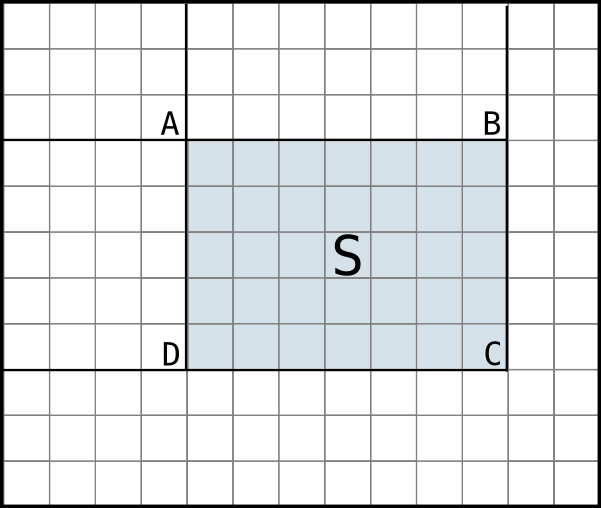
\includegraphics[width=5cm]{img/integral_image_sum.png}
    \caption{}
    \label{fig:integral_image_sum}
\end{wrapfigure}

Calcolare la somma del valore dei pixel contenuti in una regione rettangolare dell'immagine originale, con l'ausilio dell'immagine integrale, è un'operazione velocissima.

Si consideri la figura \ref{fig:integral_image_sum}: si vuole calcolare la somma del valore dei pixel nella regione $S$ evidenziata. I vertici del rettangolo saranno i punti $A:(x_1,y_1)$, $B:(x_2,y_1)$, $C:(x_2,y_2)$, $D:(x_1, y_2)$, notando che $1 \leq x_1 \leq x_2 \leq w$ e che $1 \leq y_1 \leq y2 \leq h$ \footnote{Nelle immagini raster, si iniziano a contare le colonne e le righe dal punto in alto a sinistra.}.
Quindi:

\begin{align*}
    \sum_{i = x_1}^{x_2} \sum_{j = y_1}^{y_2} I(i,j) =
    \sum_{i = 1}^{x_2} \sum_{j = y_1}^{y_2} I(i,j) - \sum_{i = 1}^{x_1} \sum_{j = y_1}^{y_2} I(i,j) = \\
    =
    \left(
    \sum_{i = 1}^{x_2} \sum_{j = 1}^{y_2} I(i,j) -
    \sum_{i = 1}^{x_2} \sum_{j = 1}^{y_1} I(i,j)
    \right)
    -
    \left(
    \sum_{i = 1}^{x_1} \sum_{j = 1}^{y_2} I(i,j) -
    \sum_{i = 1}^{x_1} \sum_{j = 1}^{y_1} I(i,j)
    \right) = \\
    = SAT(C) - SAT(B) - SAT(D) + SAT(A)
\end{align*}

Elaborare l'immagine integrale è un'operazione con complessità computazionale $\Theta(w \cdot h)$, cioè il cui costo varia linearmente con la dimensione dell'immagine. Una volta ottenuta però, permette di calcolare qualsiasi somma di pixel in regioni rettangolari con operazioni di complessità $\Theta(1)$.

Grazie all'immagine integrale è quindi possibile valutare in tempi brevi, gruppi enormi di feature sulla stessa immagine.


\section{Decision Stump}
\label{sec:decision_stump}
\begin{wrapfigure}{R}{0cm}
    \centering
    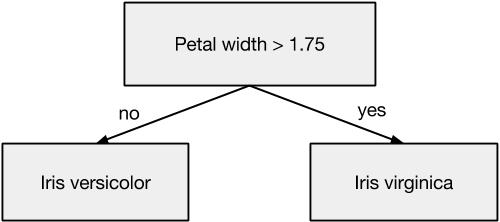
\includegraphics[width=7cm]{img/decision_stump.jpg}
    \caption{Esempio di decision stump usato per dividere gli oggetti in due classi delle tre descritte nel dataset delle caratteristiche dei fiori di Iris \cite{Fisher36}}
    \label{fig:decision_stump}
\end{wrapfigure}
Si tratta di \emph{alberi decisionali} binari di profondità unitaria.
Vi è un unico test alla radice, in base al quale si decide l'appartenenza di un oggetto ad due classi. Combinando tra loro diversi decision stump, è possibile creare alberi decisionali più complessi da poter utilizzare in alberi di classificazione non binari.

I decision stump costituiscono il meccanismo più semplice di classificazione che si può avere a disposizione. Il test da collocare alla radice dell'albero viene eseguito sul valore di una feature di Haar.

\begin{equation}
    test_1(x) =
    \begin{cases}
        true & \text{ se } f_1(x) < \theta_1\\
        false & \text{ altrimenti }
    \end{cases}
    \label{eq:decision_stump_minor}
\end{equation}

\begin{equation}
    test_2(x) =
    \begin{cases}
        true & \text{ se } f_2(x) > \theta_2\\
        false & \text{ altrimenti }
    \end{cases}
    \label{eq:decision_stump_maior}
\end{equation}

Le equazioni \ref{eq:decision_stump_minor} e \ref{eq:decision_stump_maior} descrivono due possibili test decisionali che possono essere collocati alla radice di un decision stump.
Per standardizzare la forma dei test si utilizzerà l'equazione \ref{eq:decision_stump}.

\begin{equation}
    test(x) =
    \begin{cases}
        true & \text{ se } f(x)p > p\theta\\
        false & \text{ altrimenti }
    \end{cases}
    \label{eq:decision_stump}
\end{equation}

In riferimento all'equazione \ref{eq:decision_stump}, $x$ è un'immagine di profondità, $f$ una feature di Haar ed $f(x)$ il valore della feature misurato sull'immagine $x$.
Il parametro $p \in \{ 1, -1 \}$, che assumerà il nome di \emph{polarità}, serve solamente per invertire il segno della disequazione all'occorrenza.
Il parametro $\theta$ è il valore di \emph{soglia} (\emph{threshold}).

Utilizzare i decision stump con le immagini di profondità equavale a verificare la presenza di variazioni di quota tra regioni contigue dell'immagine al di sopra o al di sotto di un certo valore di soglia.
La scelta del valore di soglia non è un problema banale e sarà trattato approfonditamente nel prossimo capitolo.

Il successo o l'insuccesso del test deve essere interpretato correttamente ai fini della classificazione. Di qui in avanti qualsiasi test decisionale applicato ad immagini di profondità che avrà successo, segnalerà la presenza di una persona, mentre, viceversa, quelli che non avranno successo ne segnaleranno l'assenza.


	% % !TEX root=../index.tex

\chapter{Adaboost}
\label{cap:adaboost}
\emph{Classificazione nell'ambito degli algoritmi di apprendimento automatico.
Costruzione e preparazione dei dataset di allenamento:
    definizione delle categorie di classificatori da utilizzare;
    operazioni preliminari di preprocessing.
Procedura di estrazione del classificatore forte.
Procedura di estrazione del miglior classificatore debole.}


Adaboost è un algoritmo di apprendimento automatico della famiglia degli \emph{ensamble learner}. Un algoritmo di ensamble learning mira alla costruzione di un classificatore composto da un insieme di


Adaboost è un \emph{meta algoritmo} di \emph{machine learning} che viene utilizzato per aumentare le prestazioni di altri algoritmi di apprendimento. Ciò avviene estraendo un \emph{classificatore forte} a partire da un insieme di \emph{classificatori deboli}, dove per classificatore si intende una funzione $f(x)$ che identifichi la \emph{classe} di appartenenza dell'oggetto $x$ in input.

La realtà d'interesse del problema prevede l'esistenza di due classi di oggetti: \emph{umano} e \emph{non umano}.

I dati in input per la fase di allenamento sono costituiti dal \emph{dataset di allenamento}, ovvero una raccolta di oggetti preclassificati attraverso i quali Adaboost riuscirà a selezionare una combinazione di classificatori deboli che meglio approssimano la classificazione degli elementi del dataset.

\subsection{Il dataset dall'allenamento} % (fold)
\label{sub:il_dataset_dall_allenamento}
La finestra di visualizzazione, come accennato in precedenza è di $512 \times 424$ pixel. In una registrazione che riprende dall'alto una persona che attraversa la stanza camminando, la figura della persona occupa una porzione della finestra di circa $160 \times 100$ pixel.

Un dataset di allenamento non è altro che un insieme di porzioni di frame di una certa dimensione (la stessa per tutti) che vegono classificati manualmente dal creatore\footnote{Il sistema di apprendimento che si sta trattando ricade nella categoria dei sistemi di \emph{apprendimento supervisionato}.} del dataset.

% subsection il_dataset_dall_allenamento (end)

\subsection{Estrazione del classificatore forte} % (fold)
\label{sub:estrazione_del_classificatore_forte}
Sia $D = \{(x_1, y_1), ..., (x_n, y_n)\}$ un insieme di $n$ coppie costituite da un'immagine ($x_i$) e la relativa classificazione ($y_i \in \{ 0, 1 \}$). Se $y_i = 1$, allora $x_i$ appartiene alla classe \emph{umano} (la coppia $(x_i, y_i)$ prende il nome di \emph{esempio positivo}), altrimenti appartiene alla classe \emph{non umano} (la coppia $(x_i, y_i)$ prende il nome di \emph{esempio negativo}).

L'insieme $D$ può essere partizionato come segue:
$$P = \{(x, y) \in D | y = 1\} \text{ e } N = \{(x,y) \in D | y = 0\}$$

Si tenga a mente che, essendo $P$ ed $N$ partizioni di $D$, valgono le seguenti\footnote{La scrittura $\#(D)$ denota il numero di elementi dell'insieme $D$.}:
\begin{equation}
    D = P \cup N
\end{equation}
\begin{equation}
    P \cap N = \emptyset
\end{equation}
\begin{equation}
    \#(D) = \#(P \cup N) = \#(P) + \#(N)
\end{equation}

Si introduce anche il concetto di \emph{classificatore debole}. Si tratta di una funzione che per una data immagine $x$ in ingresso, assume il valore che simboleggia la presunta classe di appartenenza di quest'ultima.
Nel dettaglio:
\begin{equation}
    h(x) = \begin{cases}
    1 & \text{se $pf(x) < p\theta$}\\
    0 & \text{altrimenti}
\end{cases}
\end{equation}
dove $f(x)$ è il valore di una feature di Haar applicata all'immagine $x$, $p \in \{-1,1\}$ è detta \emph{polarità} e $\theta$ è la \emph{soglia} (\emph{threshold}). Tutti i classificatori deboli sono costruiti usando un'unica feature.

L'obbiettivo di Adaboost è quello di formare un \emph{classificatore forte} come combinazione lineare dei migliori classificatori deboli estraibili dal set di allenamento, dove il fattore moltiplicativo di ogni classificatore nella combinazione è inversamente proporzionale agli errori di classificazione compiuti da quest'ultimo in fase di allenamento.

Il seguente algoritmo descrive la procedura di estrazione e combinazone di $T$ classificatori deboli.

\begin{enumerate}
    \item Si associa ad ogni elemento $(x_i, y_i) \in D$ un peso $w_i$ tale che $w_i = \frac{1}{2l}$ se $(x_i, y_i) \in P$ oppure $w_i = \frac{1}{2m}$ se $(x_i, y_i) \in N$, dove $l = \#(P)$ ed $m = \#(N)$ (numero degli esempi positivi e numero degli esempi negativi).

    Sia inoltre $n := \#(D) = \#(P) + \#(N) = l + m$.

    \item \emph{For} $t = [1:T]$
    \begin{enumerate}
        \item Si normalizzano i pesi, in modo che la loro somma sia pari ad 1:
        $$ w_{t,i} \leftarrow \frac{w_{t,i}}{\sum_{j = 1}^{n}w_{t,j}}$$

        \item \label{adaboost_minimum_error}
        Si estrae il miglior classificatore debole. La procedura viene esposta nel dettaglio nella sezione \ref{sub:il_miglior_classificatore_debole}, ma si tenga presente che il miglior classificatore è quello il cui \emph{errore pesato} è minimo per la corrente iterazione.
        $$ \epsilon_t = \min_{f,p,\theta} \{
        \sum_{i = 1}^{n} w_{t,i} \cdot |h(x_i, f, p, \theta) - y_i|
        \} $$
        Siano inoltre $f_t$, $p_t$, $\theta_t$ i parametri del classificatore debole che ne minimizzano l'errore pesato:
        $$ h_t(x) := h(x, f_t, p_t, \theta_t) $$

        \item \label{adaboost_beta} $\beta_t \leftarrow \frac{\epsilon_t}{1 - \epsilon_t}$

        \item \label{adaboost_update_weights} Si aggiornano i pesi
        $$ w_{t+1, i} \leftarrow w_{t,i} \cdot \beta_{t}^{e_i} $$
        dove $e_i = 1$ se $(x_i, h_t(x_i)) \in D$ (ovvero se $x_i$ è classificata correttamente), $e_i = 0$ altrimenti.

        \item $\alpha_t \leftarrow \log(\frac{1}{\beta_t})$
    \end{enumerate}

    \item \label{adaboost_strong_classifier} Il classificatore forte è dato da:
    \begin{equation}
        F(x) = \begin{cases}
        1 & \text{ se } \sum_{t = 1}^{T} \alpha_t h_t(x) > \theta \sum_{t = 1}^{T} \alpha_t \\
        0 & \text{ altrimenti }
    \end{cases}
\end{equation}
dove $\theta \in [0,1]$ è la soglia.
\end{enumerate}

Si noti che, nel'operazione \ref{adaboost_minimum_error}, l'errore pesato non è altro che la somma dei pesi degli esempi non classificati correttamente. Infatti:
$$ h(x_i, f, p, \theta) = y_i \Rightarrow |h(x_i, f, p, \theta) - y_i| = 0 $$
$$ h(x_i, f, p, \theta) \neq y_i \Rightarrow |h(x_i, f, p, \theta) - y_i| = 1 $$

Al punto \ref{adaboost_beta}, il valore di $\beta_t$ non è altro che il rapporto tra l'errore pesato del classificatore debole e la somma dei pesi delle immagini classificate correttamente. Tale valore è chiaramente $0 < \beta_t < 1$.

In fase di aggiornamento dei pesi (punto \ref{adaboost_update_weights}), i pesi relativi ad esempi classificati correttamente vengono moltiplicati per $\beta_t$ ($\beta_{t}^{1} = \beta_t < 1$) e quindi decrementati, mentre gli altri vengono lasciati inalterati ($\beta_{t}^{0} = 1$). Fare in modo che gli esempi non classificati correttamente abbiano un peso maggiore di quelli classificati correttamente è il modo per influenzare la scelta del classificatore debole successivo che andrà a colmare le lacune del suo predecessore.

La scelta della soglia per il classificatore forte (punto \ref{adaboost_strong_classifier}) deve minimizzare il numero di esempi classificati in modo errato.

% subsection estrazione_del_classificatore_forte (end)

\subsection{Il miglior classificatore debole} % (fold)
\label{sub:il_miglior_classificatore_debole}
Si è detto che un classificatore debole è costruito a partire da una feature di Haar. La scelta del migliore, quindi, mira ad identificare la feature, la polarità e la soglia che minimizzano l'errore pesato di classificazione.

Si ricordi che le feature di Haar sono degli indicatori di quanto le intensità dei pixel variano da una regione della feature ad un'altra. Il classificatore debole, quindi, classificherà l'immagine a seconda che tale indice sia maggiore o minore di una certa soglia. Il compito della polarità è quello di stabilire il verso della diseguaglianza.

Il pool di feature da testare è costituito - teoricamente - da tutte quelle individuabili nell'immagini di allenamento. Nell'opera di Viola e Jones vengono utilizzate immagini di allenamento di $24 \times 24$ pixel e 5 tipologie di feature (\cite{Viola04}, sezione 2.2): il numero di possibili features in tale area è maggiore di 160000. In questa applicazione si utilizzano immagini di $160 \times 100$ pixel e 4 tipologie di feature: il pool è costituito da un numero di elementi maggiore di almeno 4 ordini di grandezza.

È da tener presente che moltissime di queste feature sono poco significative in questa situazione: non ha senso calcolare la variazione di intensità di due aree molto piccole con delle immagini che hanno una risoluzione tanto alta. Effettuando una prima scrematura, si cercherà di avere un pool di feature selezionabili la cui dimensione non superi quella del pool di Viola-Jones per più di un ordine di grandezza.

Sia $\{ f_1,...,f_k\}$ l'insieme di tutte le feature selezionabili, $D = \{(x_1,y_1), ..., (x_n, y_n) \}$ l'insieme degli esempi di allenamento e $\{w_1, ..., w_n\}$ l'insieme dei relativi pesi. La scelta del classificatore debole avviene come descritto dal seguente algoritmo in pseudocodice:

\begin{enumerate}
    \item Si calcolano $T^+$ e $T^-$, rispettivamente, somma dei pesi degli esempi negativi e di quelli negativi:
    $$T^+ \leftarrow \sum_{i = 1}^{n} (w_i y_i)
    \text{ , }
    T^- \leftarrow \sum_{i = 1}^{n} [w_i (1 - y_i)]$$

    \item \emph{For} $f = [f_1, ..., f_k]$

    \begin{enumerate}
        \item Si inizializza una lista di $n$ elementi per memorizzare i valori della feature i-esima applicata ad ogni immagine di allenamento:
        $$values[i] \leftarrow f(x_i) \; \forall x_i \in D$$

        \item Si ordinano gli elementi della lista in ordine crescente. Si tenga in conto che, dopo tale operazione, all'i-esima posizione della lista non corrisponderà più il valore della feature applicata all'i-esima immagine di allenamento.

        \item Si inizializzano $S^+$ ed $S^-$, con le quali, scorrendo gli elementi della lista con un cursore, indicheremo rispettivamente la somma dei pesi degli esempi positivi e di quelli negativi: $S^+ \leftarrow 0, S^- \leftarrow 0$

        \item \emph{For} $i = [1:n]$

        \begin{enumerate}
            \item A causa del rilocamento degli indici, alla posizione i-esima della lista corrisponderà il valore della feature dell'elemento $x_j$ con classificazione $y_j$ e peso $w_j$ tale che $(x_j, y_j) \in D$:
            $$x_j, y_j, w_j \Leftarrow values[i]$$

            \item \emph{If} $y_i = 1$ \emph{Then}
            \begin{enumerate}
                \item $S^+ \leftarrow S^+ + w_j$
            \end{enumerate}
            \item \emph{Else}
            \begin{enumerate}
                \item $S^+ \leftarrow S^- + w_j$
            \end{enumerate}

            \item \label{best_classifier_p_theta}
            Si calcola calcola l'errore pesato di classificazione:
            $$e_i = \min\{ S^+ + (T^- - S^-), S^- + (T^+ - S^+) \}$$

        \end{enumerate}

        \item Si determinano la polarità ($p_f$) e la soglia ($\theta_f$) per cui l'errore pesato ($\epsilon_f)$ di classificazione per un classificatore che utilizza la feature $f$ è minimo:
        $$p_f, \theta_f | \epsilon_f = \min \{ e_1, ..., e_n \}$$
    \end{enumerate}

    \item Si scelgono polarità ($p$) e soglia ($\theta$) finali, ovvero quelle del classificatore debole con errore pesato $\epsilon$ minore tra tutti i classificatori possibili:
    $$p, \theta | \epsilon = \min \{ \epsilon_1, ..., \epsilon_k \}$$
    Il miglior classificatore debole è quindi:
    \begin{equation}
        \label{eq:weak_classifier}
        h(x) := \begin{cases}
        1 & \text{ se } pf(x) < p\theta \\
        0 & \text{ altrimenti }
    \end{cases}
\end{equation}

\end{enumerate}

Il metodo di identificazione della polarità e della soglia non viene riportato nell'algoritmo, essendo un passaggio che merita una trattazione a parte. Selezionare un valore di soglia vuol dire trovare il \emph{punto che partiziona al meglio la lista dei valori della feature calcolata sulle immagini di allenamento, in modo tale da minimizzare gli errori di classificazione}. La miglior soglia di una buona feature fa in modo che la maggior parte delle immagini appartenenti alla stessa classe assumano un valore minore (o maggiore). Si può notare, come diretta conseguenza, che con una feature pessima per la classificazione non sarà possibile trovare un valore di soglia che soddisfi tale criterio.

Al punto \ref{best_classifier_p_theta} viene calcolato l'errore pesato di classificazione per una feature $f$ con soglia $values[i]$\footnote{I possibili valori delle soglie corrispondono esattamente ai valori della feature calcolata sugli esempi di allenamento}. Per essere più espliciti, bisogna effettuare una serie di osservazioni:
\begin{enumerate}
    \item \label{obs:1} $T^+$ ($T^-$) corrisponde alla somma dei pesi degli esempi positivi (negativi);
    \item \label{obs:2} $S^+$ ($S^-$) corrisponde alla somma dei pesi degli esempi positivi (negativi) dalla prima posizione fino all'i-esima della lista (quella su cui è posizionato il cursore);
    \item \label{obs:3} $T^+ - S^+$ ($T^- - S^-$) corrisponde alla somma dei pesi degli esempi positivi (negativi) dalla posizione $i+1$ della lista fino alla fine;
    \item \label{obs:4} Per un classificatore della forma (\ref{eq:weak_classifier}) con $p = 1$, $S^+$ corrisponde alla \emph{somma dei pesi degli esempi classificati correttamente}, mentre $S^- + (T^+ - S^+)$ corrisponde alla somma dei pesi degli esempi classificati in modo scorretto;
    \item \label{obs:5} Per l'osservazione \ref{obs:4} un classificatore (\ref{eq:weak_classifier}) con $p = 1$, la quantità $S^- + (T^+ - S^+)$ è \emph{l'errore pesato};
    \item \label{obs:6} Analogamente alle osservazioni \ref{obs:4} e \ref{obs:5}, un classificatore (\ref{eq:weak_classifier}) con $p = -1$ commetterà un errore pesato pari alla quantità $S^+ + (T^- - S^-)$.
\end{enumerate}

Grazie alle osservazioni \ref{obs:5} e \ref{obs:6}, dal semplice calcolo dell'errore di classificazione pesato, si ottiene anche il valore della polarità:
\begin{equation}
    p = \begin{cases}
    1 & \text{ se } S^- + (T^+ - S^+) < S^+ + (T^- - S^-) \\
    -1 & \text{ altrimenti }
\end{cases}
\end{equation}

In definitiva, con uno scorrimento della lista ordinata si ottengo i parametri per la costruzione del classificatore debole. La complessità di tale operazione è fortemente legata all'algoritmo di ordinamento della lista, la quale ha $\Theta(n\log n)$ come limite teorico inferiore \cite[p. 167]{Cormen09}. Nell'implementazione è stato scelto proprio un algoritmo che avesse complessità $\Omega(n\log n)$ nel caso peggiore. Ripetendo queste operazioni per ognuna delle feature selezionabili, si ottiene che l'algoritmo di selezione del miglior classificatore debole ha complessità $\Theta(kn\log n)$.

% subsection il_miglior_classificatore_debole (end)

% section adaboost (end)


	% \chapter{Tuning}
	% \label{chap:Tuning}
	% \emph{Definizione dei criteri di valutazione delle prestazioni.
	% Algoritmo di massimizzazione dell'accuratezza.
	% Valutazione del risultato dell'algoritmo di apprendimento.
	% Valutazione degli elementi di disturbo.}
	%
	% \chapter{Rilevamento}
	% \label{chap:Rilevamento}
	% \emph{Presentazione della tecnica di rilevamento su registrazioni reali.
	% Algoritmo evoluto di selezione della finestra ottima.
	% Tecniche di ottimizzazione dell'operazione di rilevamento a regime.
	% Presentazione e confronto dei risultati ottenuti con quelli in letteratura.}
	%
	% \chapter{Conclusioni}
	% \label{chap:Conclusioni}
	%
	% \begin{appendices}
	%
	% 	% !TEX root=../index.tex

\chapter{Software Sviluppato}
\label{chap:software}
    \section{Componenti}
        \subsection{Gestore dei Dataset} % (fold)
        \label{sub:training_set_creator}
            \subsubsection{Interfaccia Grafica}
            \subsubsection{Strutture Dati per la persistenza}
            \subsubsection{Tecnologie utilizzate}        
        % subsection training_set_creator (end)
        
        \subsection{Allenamento}
            \subsubsection{Punti critici dal punto di vista computazionale}
            \subsubsection{Mex files}
            \subsubsection{Architettura delle librerie}
            \subsubsection{Struttura dati per la persistenza}
        \subsection{Tuning, Testing, Rilevamento}
            \subsubsection{Organizzazione degli script e delle funzioni}
            \subsubsection{Struttura dati per la persistenza}
    \section{Tecnologie utilizzate}
        \subsection{C++ e Matlab}
            \subsubsection{Matlab: prototipazione e componenti non critiche}
            \subsubsection{C++: ottimizzazione delle componenti critiche}
        \subsection{Git e Github [Opzionale]}
            \subsubsection{Sistemi VCS}
    \section{Proposte di miglioramento}
        \subsubsection{Componenti da ottimizzare}
        \subsubsection{Nuovi linguaggi da utilizzare}
	%
	% 	% !TEX root=../index.tex

\chapter{Cenni sul Funzionamento del Sensore del Kinect} % (fold)
\label{cha:kinect}

% chapter kinect (end)
	%
	% \end{appendices}

	% Far comparire tutti gli elementi della bibliografia
	\nocite{*}
	\bibliographystyle{plainnat}
	\bibliography{bibliografia}{}

\end{document}
